\documentclass[notitlepage]{report}

\title{
	\textsc{ \small
		Physics 415
	} \\
	{\textsc{\small Lab \#1}} \\
	Michelson Interferometry
}
\author{Kevin Evans \\ Partner: Sierra Ray}
\date{February 16, 2021}
\usepackage{amssymb}
\usepackage{mathtools}

\usepackage{amsthm}
\usepackage{amsmath}
\usepackage{slashed}
\usepackage{relsize}
\usepackage{threeparttable}
\usepackage{float}
\usepackage{booktabs}
\usepackage{boldline}
\usepackage{changepage}
\usepackage{physics}
\usepackage[inter-unit-product =\cdot]{siunitx}
\usepackage{setspace}
\usepackage{caption}
\usepackage{subcaption}
\usepackage[makeroom]{cancel}
%\usepackage{pgfplots}

\usepackage{enumitem}
\usepackage{times}
\usepackage{titling} % for titlingpage environment
\usepackage{calligra}
\usepackage{graphicx}
\DeclareMathAlphabet{\mathcalligra}{T1}{calligra}{m}{n}
\DeclareFontShape{T1}{calligra}{m}{n}{<->s*[2.2]callig15}{}
\newcommand{\scriptr}{\mathcalligra{r}\,}
\newcommand{\boldscriptr}{\pmb{\mathcalligra{r}}\,}
\newcommand{\emf}{\mathcal{E}}
\renewcommand{\thesection}{\arabic{section}}

\begin{document}
	\begin{titlingpage}
		\maketitle
		\begin{abstract}
			\noindent A Michelson interferometer was constructed with a HeNe laser. An interference pattern was verified and the laser wavelength was calculated by finding fringe changes per distance. The wavelength was found to be $\left(\num{656.0} \pm \num{20}\right) \si{\nm}$, somewhat beyond the expected value of \SI{632.8}{\nm}. The laser light was replaced with a red, and later white, LED and the coherence lengths were calculated. The coherence lengths for the red and white LED were found to be $\ell_c = \SI{33.2}{\um} \pm \SI{0.5}{\um}$ and $\SI{6.9}{\um} \pm \SI{0.5}{\um}$ respectively. The line width of the red LED was found to be $(9.03 \pm 0.136) \; \si{\THz}$, short of the expected \SI{15.1}{\THz}.
		\end{abstract}
	\end{titlingpage}

	\section{Description of Experiment}
	In this experiment, the behavior of the Michelson interferometer was verified. A Michelson interferometer was built on a broadboard using a HeNe ($\lambda = \SI{632.8}{\nm}$) laser. One arm of the interferometer reflected using a retromirror on a translation stage (mirror RM1), adjustable by a total \SI{2}{\mm} with \SI{1.0}{\um} ticks. % ticks? or precision. graduations?
	The secondary retromirror (RM2) was mounted in a fixed stage and adjustable on two rotation axes. Each arm was \SI{9.0}{\centi\meter} from a beam-splitter cube (BSPC). The interferometer setup is shown below in Figure \ref{fig:lab1diagram}. A divergence lens ($f=\SI{50}{\mm}$) was placed in front of the beam-splitter cube. Initially, the translatable mirror RM1 was adjusted such that an interference pattern was shown on the screen, shown in Figure \ref{fig:interference}. A beam-splitter plate (BSPP) was placed between the lens and BSPC, creating a second interference pattern on the screen. An estimation of the laser wavelength was determined experimentally. This was done by slowly adjusting the translation stage until the fringe pattern changed 50 times.
	
	The HeNe laser was then replaced with a red LED and mirror RM2 was adjusted such that the secondary arm was within a millimeter of the primary arm length. This created an interference pattern on the screen due to the incident LED light. The range of the translation stage, over which the interference pattern was visible, was measured and an estimation of the red coherence length was measured. The red LED was replaced with a white LED, and an estimation of the white LED coherence length was measured.
	

	\begin{figure}[p]
		\centering
		\begin{subfigure}[b]{0.5\textwidth}
			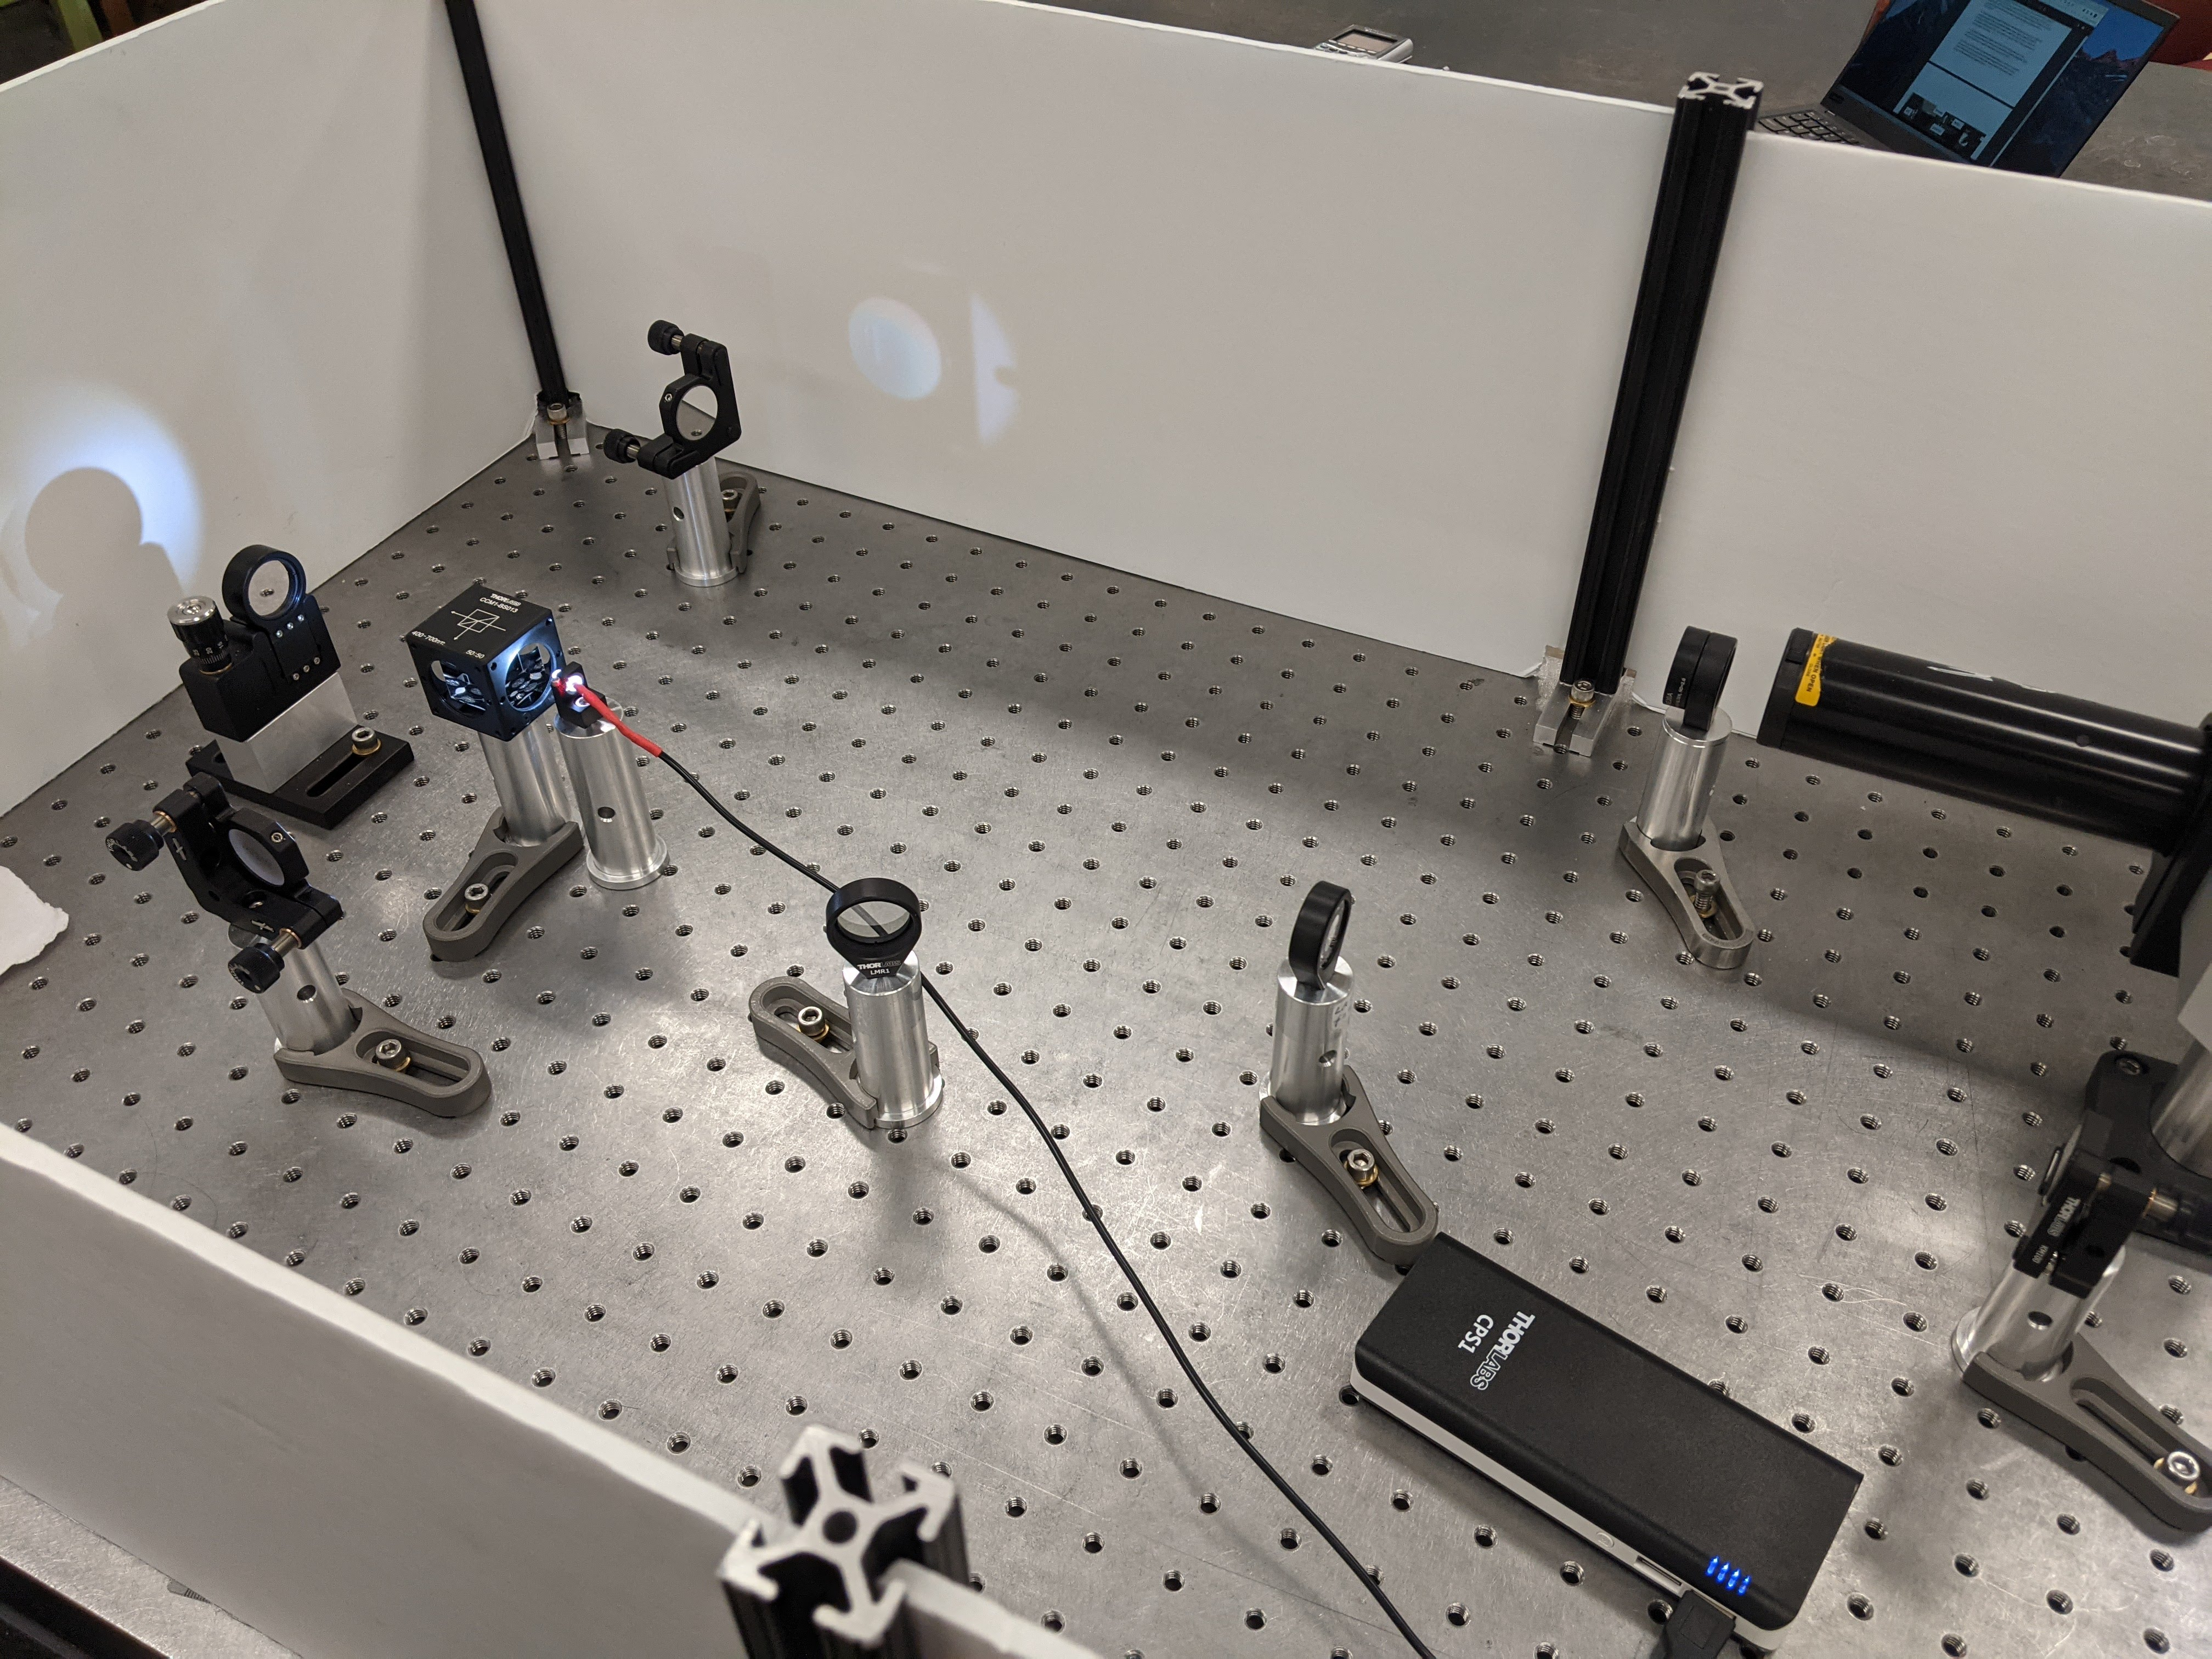
\includegraphics[width=\linewidth]{PXL_20210205_010019887}
		\end{subfigure}
		\hfill
		\begin{subfigure}[b]{0.45\textwidth}
			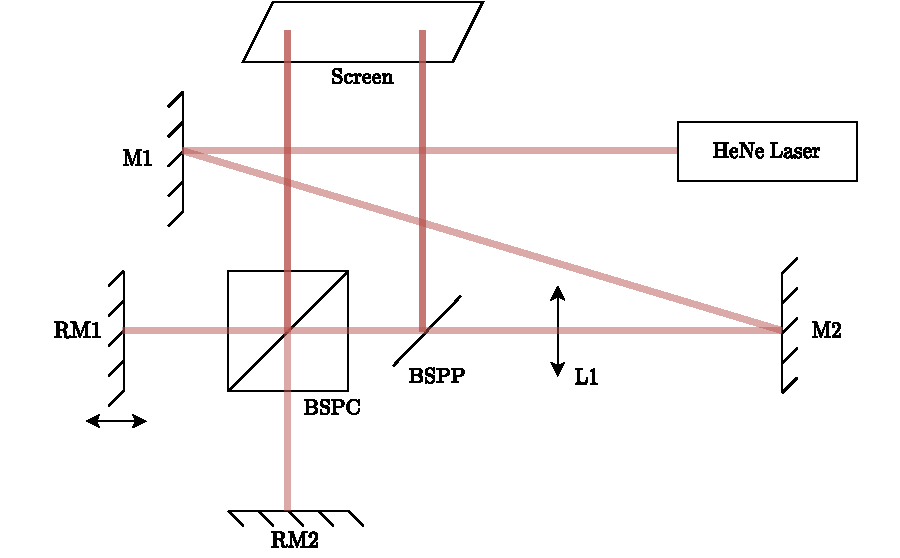
\includegraphics[width=\linewidth]{lab1diagram}
		\end{subfigure}
		\caption{An image (left) and diagram (right) of the Michelson interferometer setup.}
		\label{fig:lab1diagram}
	\end{figure}
	
	
	\begin{figure}[p]
		\centering
		\begin{subfigure}[b]{0.49\textwidth}
			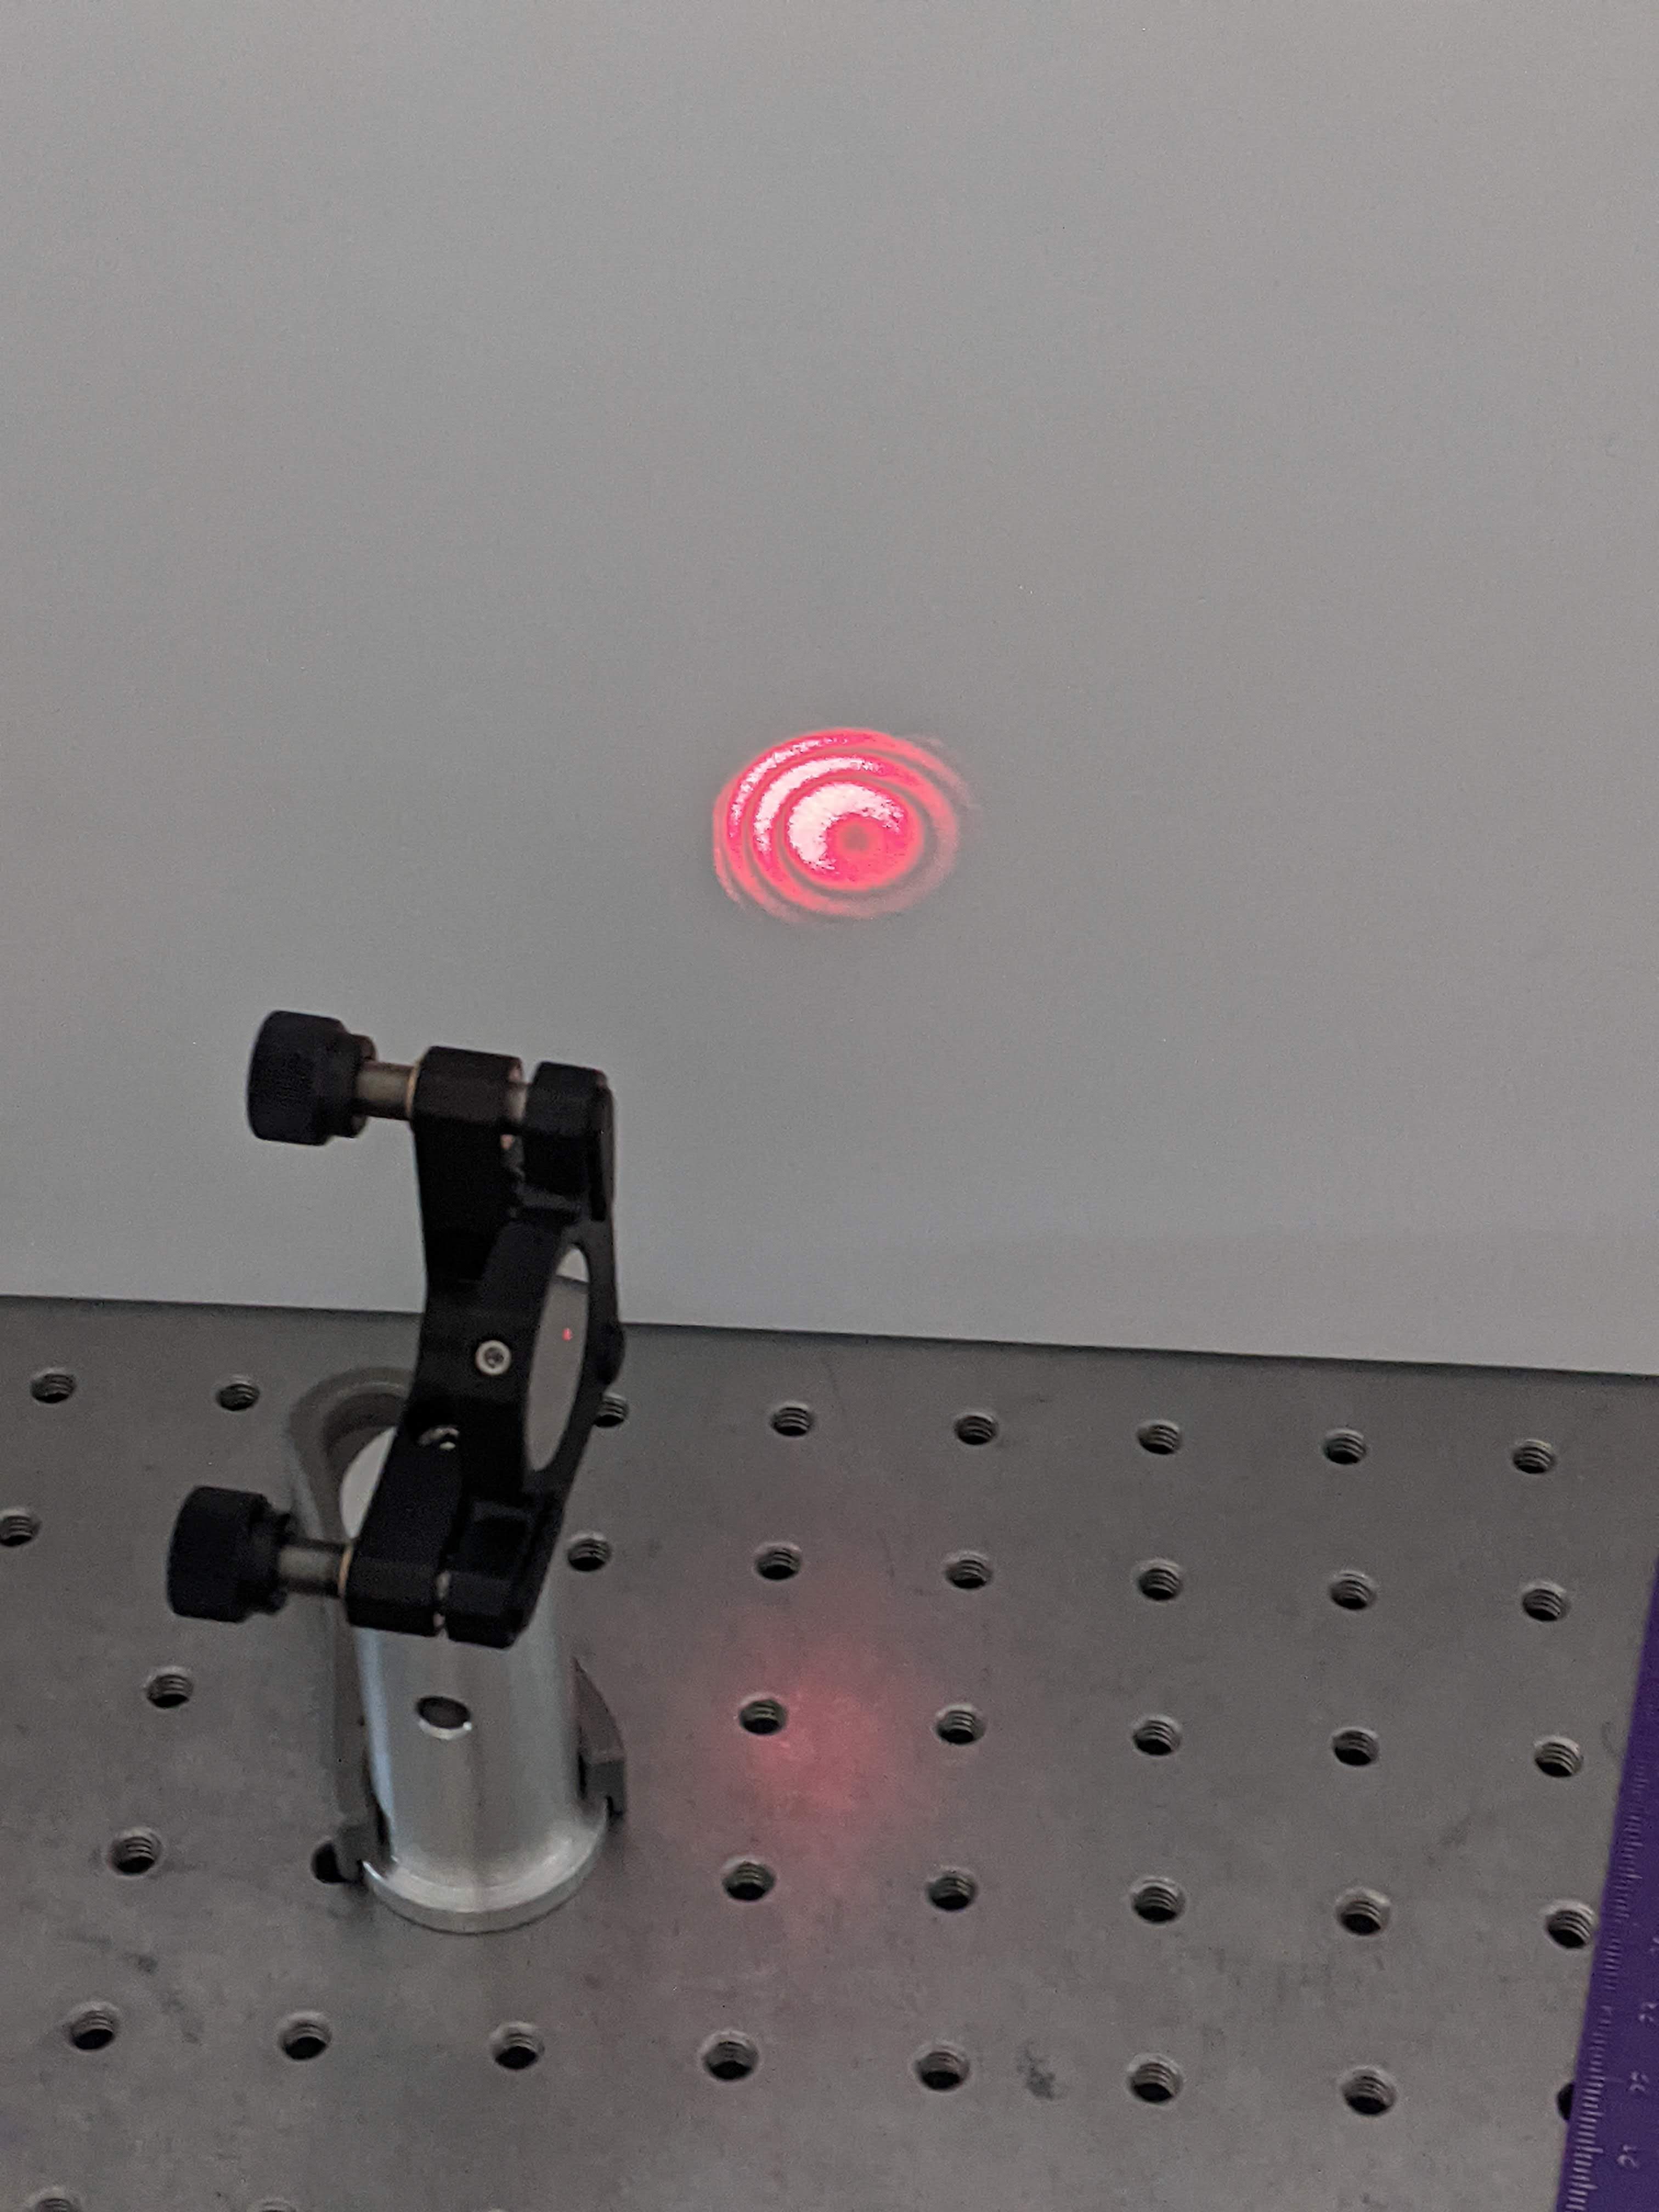
\includegraphics[width=\linewidth]{PXL_20210204_220939936}
			\caption{The interference pattern on the screen.}
			\label{fig:interference}
		\end{subfigure}
		\hfill
		\begin{subfigure}[b]{0.49\textwidth}			
			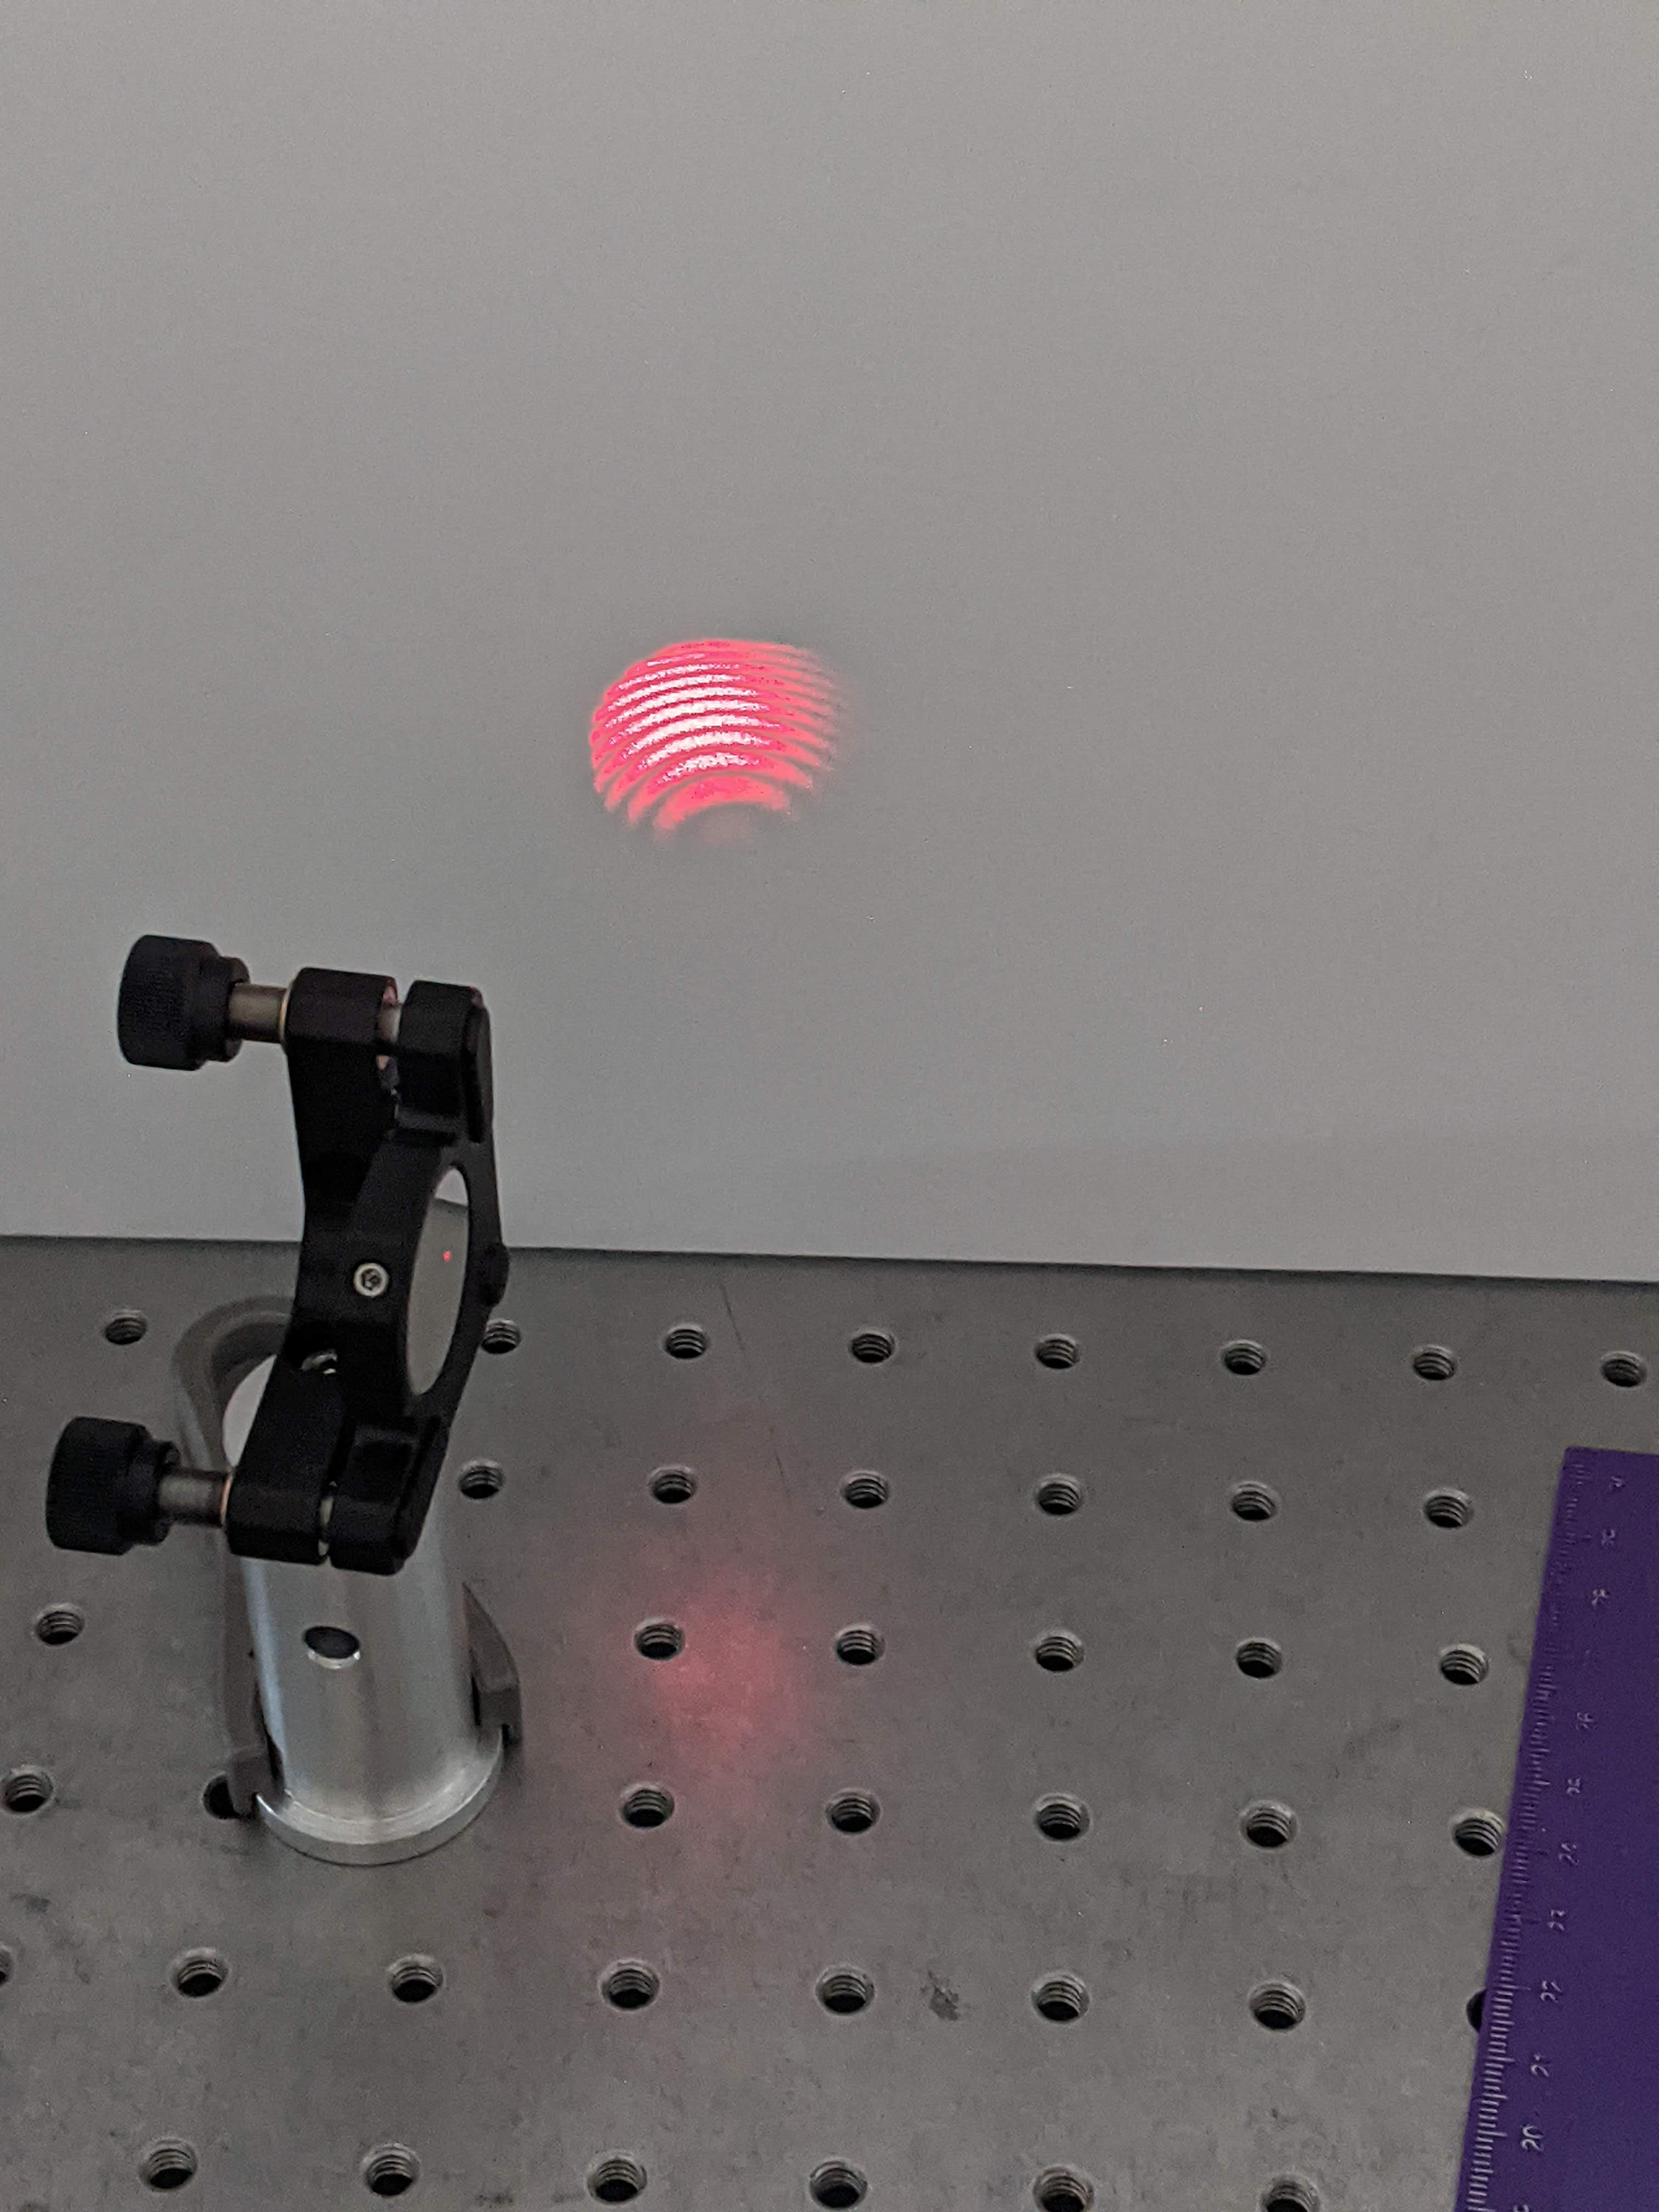
\includegraphics[width=\linewidth]{PXL_20210204_220945838}
			\caption{The screen after adjusting RM2.}
			\label{fig:interferencetweaked}
		\end{subfigure}
		\caption{The interference pattern created by the Michelson interferometer.}
		\label{fig:rm2adjustment}
	\end{figure}

	
	\section{Data and Analysis}
%	\subsection{HeNe laser qualitative analysis}
	
	By adjusting the rotation axes of RM2, it adjusts the location of the central beam on the screen, i.e.  translating the center of the Airy pattern. These changes are shown below in Figure \ref{fig:rm2adjustment}. Adjusting RM2 changes the angle of the reflected beam, in turn creating a condition where the phase of the reflected light is a function of the angle adjustments of RM2. 
	
	Similarly, adjusting the distance between RM2 and the BSPC affected the phase of one of the output beams. Since moving the retromirror adds or subtracts roughly a millimeter of path length, it effectively randomizes the phase and pattern on the screen.
	
	Adding the beam splitter plate created a second pattern on the screen, an inverse of the first pattern, shown in Figure \ref{fig:split}. This second pattern is opposite of the first pattern as it is effectively the output of the second port of the interferometer, i.e. the destination of the photons meant for the dark fringes of the original pattern.
	
	\begin{figure}[h]
		\centering
		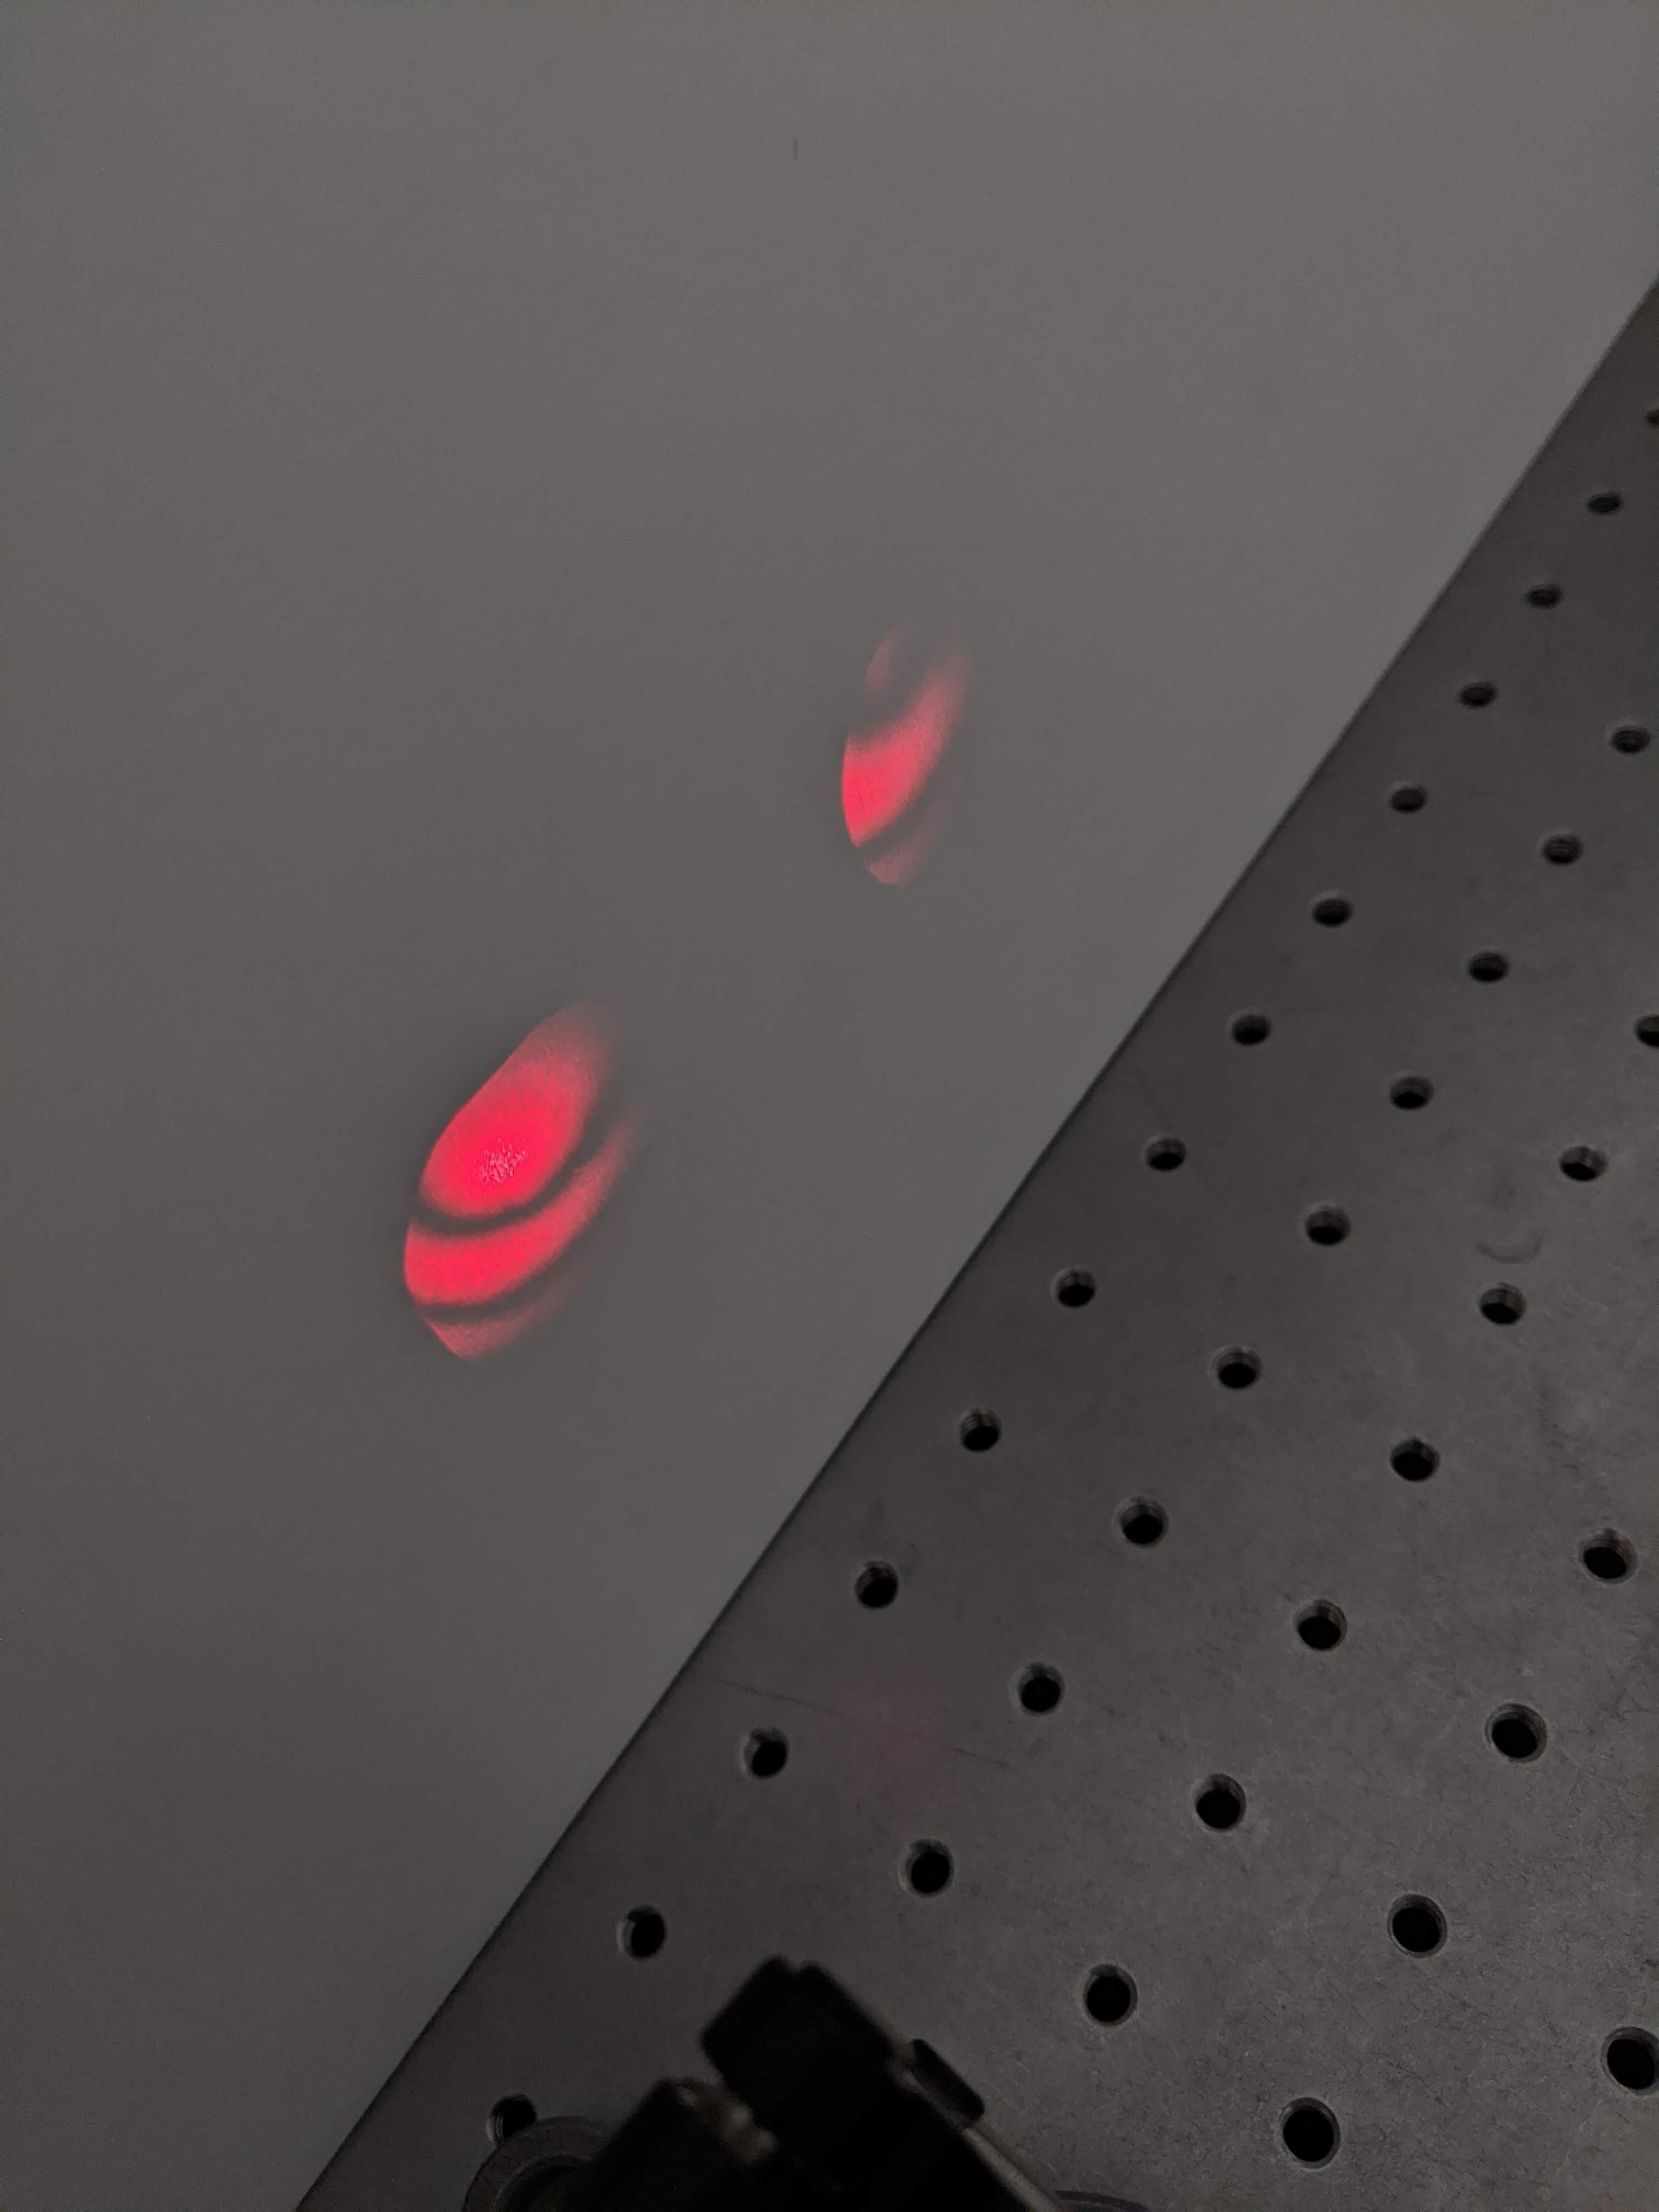
\includegraphics[width=0.5\linewidth]{PXL_20210204_222253776}
		\caption{The two opposite interference patterns created by the interferometer and beam splitter plate.}
		\label{fig:split}
	\end{figure}
	
	
	\subsection{HeNe laser wavelength estimation}
	After counting fifty fringe changes, the translation stage was shifted $\SI{16.4}{\um} \pm \SI{0.5}{\um}$\footnote{Afterwards, I realized that I think we were supposed to do multiple trials of this, but we only had done a single trial.}. As the light is reflected off the mirror and back into the beam splitter cube, the total roundtrip change in path length is $$\Delta x = \SI{33.2}{\um} \pm \SI{1.0}{\um}$$
	Dividing by the fifty fringes will give us an estimation of the wavelength and error. This results in a wavelength of $\SI{656.0}{\nm} \pm \SI{20}{\nm}$. 
	
	\subsection{LED coherence length estimation}
	The coherence lengths of the LEDs was estimated by adjusting the translation stage on RM1 until the fringes would disappear. The red LED was estimated to have $\ell_c = \SI{33.2}{\um} \pm \SI{0.5}{\um}$. 
	The line width can be calculated as \begin{align}
		\Delta \nu & = \frac{c}{\ell_c} = \frac{c\Delta \lambda}{\lambda^2} \label{eq:linewidth}
	\end{align}
	For the spectral width of \SI{20}{\nm} and assuming \SI{630}{\nm} light, the expected line width is \SI{15.1}{\THz}. The line width was found to be $(9.03 \pm 0.136) \; \si{\THz}$. After replacing the red LED with a white LED, the coherence length was found to be $\ell_c = \SI{6.9}{\um} \pm \SI{0.5}{\um}$. 
	
	\section{Results and Conclusion}
	The HeNe laser was found to have a wavelength of $$\lambda = \SI{656.0}{\nm} \pm \SI{20}{\nm}$$
	The expected value was \SI{632.8}{\nm}. The discrepancy can be explained by human error: since the fringe pattern was changing quickly, it was possible to miscount this number. If instead, there were $52$ fringes counted, it would result in an experimental wavelength of \SI{631}{\nm}. To prevent this in the future, additional trials should have been completed. 
	
	
	\subsubsection{Coherence lengths of the red and white LEDs}
	The coherence lengths for the red and white LEDs were calculated to be $\ell_c = \SI{33.2}{\um} \pm \SI{0.5}{\um}$ and $\SI{6.9}{\um} \pm \SI{0.5}{\um}$ respectively. For the red LED, the line width was calculated as $(9.03 \pm 0.136) \; \si{\THz}$, far from the expected \SI{15.1}{\THz} line width.
	
	
	There were several sources of error for these calculations. The changing fringes were hard to distinguish by eye, as the contrast becomes subtle near the coherence width edges. Future experiments could utilize an electronic method to remove the bias and shortcomings of the human eye. 
	
	While adjusting RM1 with the white LED, the interference pattern consisted of several colors visible in Figure \ref{fig:whiteinterference}, particularly violent, blue, and red. This is likely since white LEDs do not produce white light, but rather emit several peaks in its spectral power distribution, resulting in the appearance of white light. Additionally, this may explain why the coherence length was much shorter for the white LED. Since there are high energy wavelengths in the white light, the coherence length will be shorter, as $\ell_c \propto \lambda \propto \nu^{-1}$. The constituent violets and blues would contribute to this.
	
	
	\begin{figure}[h]
		\centering
		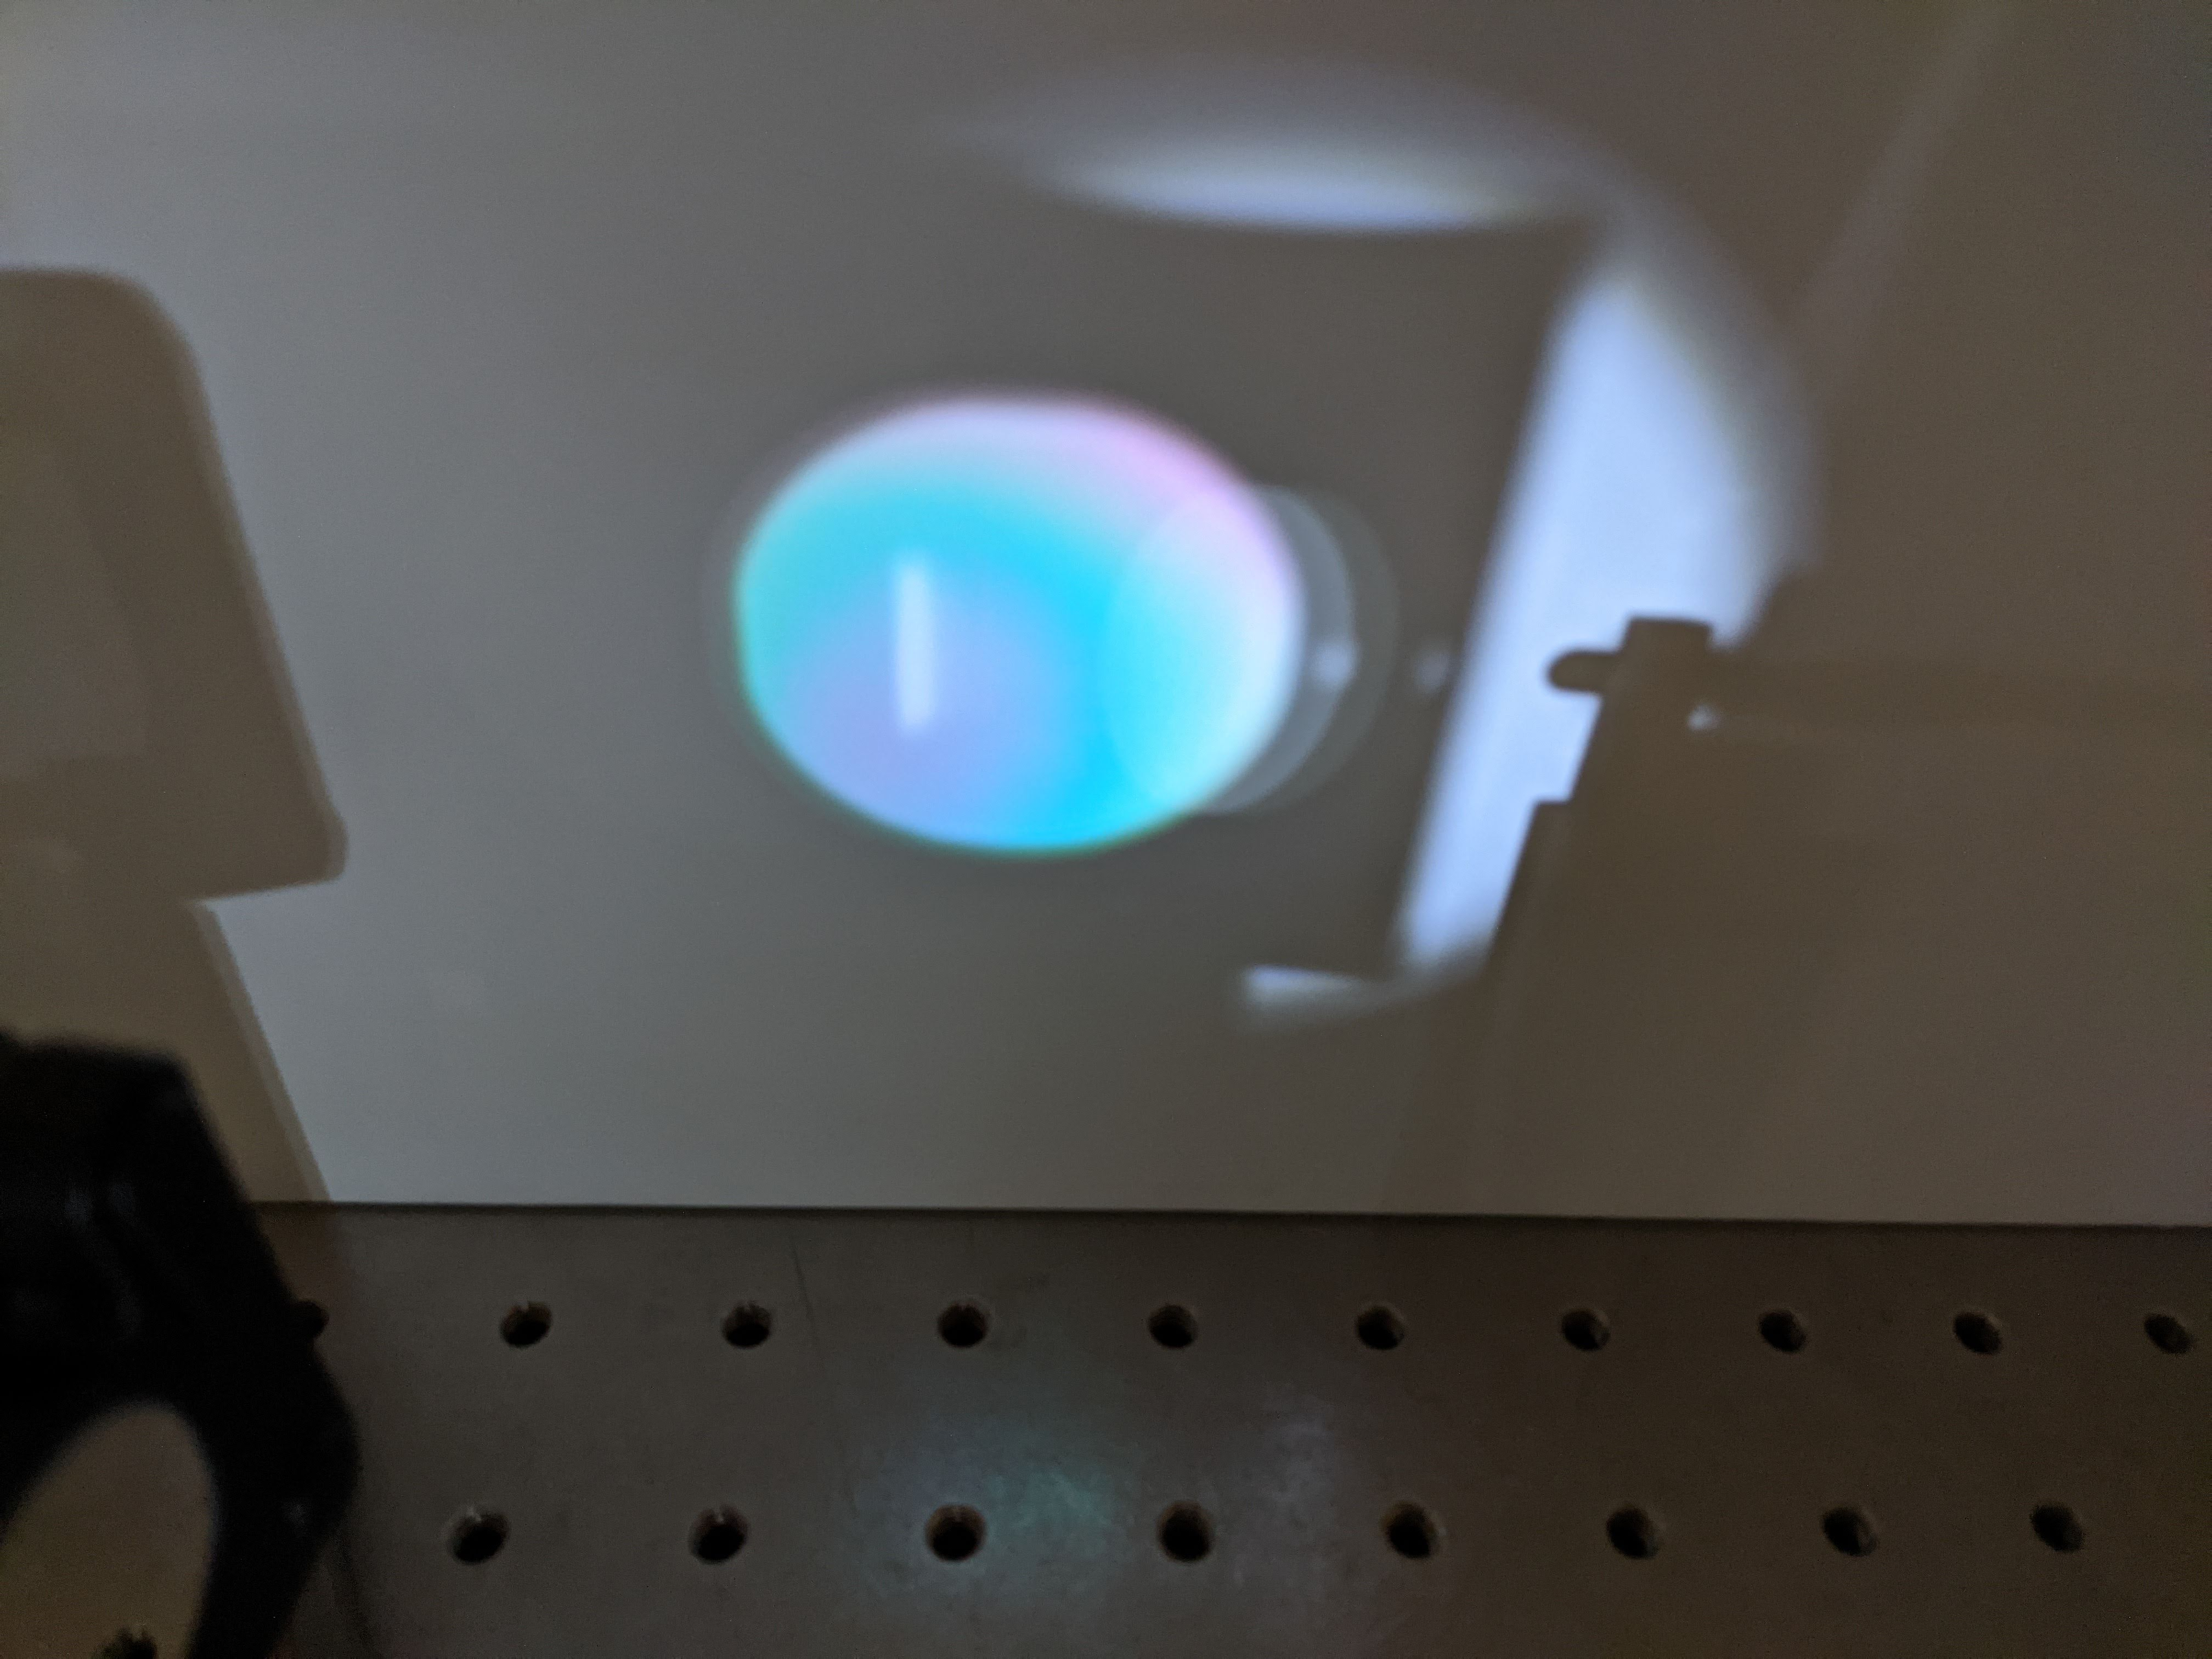
\includegraphics[width=0.5\linewidth]{PXL_20210205_005820272}
		\caption{Multicolor interference pattern created by the white LED.}
		\label{fig:whiteinterference}
	\end{figure}
	
	\newpage
	\section*{Data tables}
	\begin{table}[h]
		\caption{Translation stage (RM1) readings and calculations.}
		\begin{center}			
			\begin{tabular}{lccc}
				\toprule
				Experiment & $x_i$ (\si{\um}) & $x_f$ (\si{\um}) & $\Delta x$ (\si{\um}) \\
				\midrule
				HeNe wavelength est. & $0.0$ & $16.4$ & $16.4$ \\
				Red $\ell_c$ & $13.8$ & $47.0$ & $33.2$ \\
				White $\ell_c$ & $22.5$ & $32.4$ & $6.9$  \\
				\bottomrule
			\end{tabular}
		\end{center}
	\end{table}
\end{document}